\chapter{Introduction}
\label{cha:intro}
%Problem, motivation and significance
%TODO the origin of neuromorphic computing
%Neuromorphic computing has lead towards the development of biologically-inspired computer architectures 
Advances in computing power and machine learning have endured computers with a rapidly growing performance in cognitive tasks such as recognising objects~\citep{deng2009imagenet} and playing GO~\citep{silver2016mastering}. 
These tasks were once dominated by human intelligence and solved by biological neurons in the brain.
However, humans and many other animals still win against computers in practical tasks, such as vision, and outperform them in terms of size and energy cost by several orders of magnitude.
For instance, AlphaGO~\citep{silver2016mastering} consumed 1~MW of power on its 1920 CPUs and 280 GPUs when playing the game with one of the best human players whose brain only consumed about 20~W.
Although we are still far from understanding the brain thoroughly, it is believed that the performance gap between computation in the biological nervous system and in a computer lies in the fundamental computing units and how they compute.
Computers employ Boolean logic and deterministic digital operations based usually on synchronous clocks while nervous systems employ parallel, distributed, event-driven, stochastically unreliable components~\citep{indiveri2009artificial}: neurons.
These impressive disparities in cognitive capabilities and energy consumption drives research into biologically-plausible spiking neurons and brain inspired computers, known as Neuromorphic Engineering~(NE).

\begin{quotation}
	``As engineers, we would be foolish to ignore the lessons of a billion years of evolution.'' - Carver Mead, 1993
\end{quotation}

%Today	we	stand	poised	on	the	brink	of	a	new	era	of	compu:ng	in	which	technology	is	more	
%consumable,	insight-driven	and	cogni:ve.	IBM	Research	is	exploring	and	developing	the	
%enabling	technologies	that	will	transform	the	way	computers	are	used	
%Ginni	Rome]y	
%IBM	President,	Chairman	and	CEO	

%Two aims
NE was proposed by Carver Mead in the late 1980s \citep{Mead:1989:AVN:64998} to build analogue circuits that mimic biological neural cells and the architecture of the nervous system using Very-Large-Scale Integration (VLSI) technology.

The objectives of NE can be summarised as follows~\citep{furber2007neural}:
\begin{itemize}
	\item neuromorphic modelling: for neuroscientists to understand the brain by modelling and simulating the activities of biological neurons; 
	\item neuromorphic computing: for engineers to build brain-like machines by applying biological principles to computers.
\end{itemize}
This is a bidirectional process; building a biologically inspired computer requires a better understanding of the brain, and simulating brain activities at large scale and in real time is feasible only on massively-parallel neuromorphic hardware.

%Since around 2004 to 2005, `Dennard's Law' has no longer been followed~\citep{bohr200730}, so as transistors get smaller their power density no longer stays constant but starts to increase.
%The breakdown of Dennard scaling and the problem of power dissipation drove chip manufacturers to multi/many-core architecture.
%However, the increased number of active transistors in a multi-core chip costs more power consumption thus creating the prospect that some fraction of the cores will have to remain completely powered-off given the thermal design power constraint.
%Dark silicon~\citep{esmaeilzadeh2011dark} addresses the issue of inactive areas of a multi-core chip, which could be 50\% of nodes in an 8~nm technology.
%Neuromorphic engineering offers a potential solution for power dissipation by applying the biological features of event-driven, hybrid analogue/digital, unreliable components to computers.
%Moreover, most of the neural interconnections in the brain are local, and the `memory' units attach to the `computation' node in a neuron.
%Therefore, learning from biology may give computers an alternative to the conventional Von Neumann architecture and thus may solve the problem of the microprocessor/memory performance gap~\citep{wulf1995hitting}, also known as the Von Neumann bottleneck, where the system speed is determined and limited by the memory performance.

%Why SNN
Spiking Neural Networks (SNNs), comprised of spiking neurons, hold the key to address the dual aims of understanding brain functions and building brain-like machines.
The spiking neuron mathematically models the dynamics of a single neuron with biological realism and the network describes the architecture of the neural connections and the information transmission among them.
Therefore, neuroscientists are able to reproduce the recorded neural dynamics and activities from \textit{in-vivo/vitro} experiments of varies network sizes to verify their models and measure the progress of brain understanding;
while computer engineers can focus on the hardware implementations of the spiking neurons and the interconnections between them to build energy-efficient neuromorphic hardware.

%TODO Problem of SNN why not in engineering.
Simulations of massive SNNs have proved to be useful in neuroscience~\citep{markram2006blue,ananthanarayanan2009cat}, and the NE hardware systems have successfully decreased the power consumption of conventional SNN simulations on supercomputers~\citep{de2010world,sharp2012power}.
However, SNNs are not (yet) widely used in functional simulations of cognitive tasks.
Although SNNs can in principle be used for AI tasks the same way as traditional artificial neural networks~(ANNs), there is a major difference between the theoretical power of SNNs and what has been demonstrated.
There are two significant problems prohibiting intelligent SNNs from developing: first, the computation cost for simulating large SNNs of size as big as commonly-used ANNs;
second, it is difficult to transform ANN models to SNN algorithms which are defined in discrete time.
Therefore it is relatively easy to construct a spiking neural network model and observe its dynamics in use of neuroscience, but much harder to develop a model with stable behaviour that computes a specific function in intelligent applications.



%The SNN simulations of brain models `quantitatively simulate the generic behaviour and internal dynamics of a certain subsystem of the brain, but without precisely functionally simulating that subsystem~\citep{de2010world}.'
%Simulations NE are working well and better fitted than supercomputer and etc.
%TODO non-Von Noman




The ultimate goal of NE is to equip neuromorphic machines with genuine intelligence~\citep{konar1999artificial}.
Today, in neuromorphic computing, massive large-scale SNN hardware simulators are ready to use.
%Unfunctional
However, in neuromorphic modelling, we know that information processing in the brain is conducted by the basic computing units, the spiking neurons.
Information transmission takes place in the synapses and we can draw the connections among neurons from anatomical experiments.
%Functoinal
However, due to the fundamental difference of data representation and neural computation between spiking and artificial neurons, understanding how to operate these brain-like machines to be competent in cognitive applications still remains unsolved.

Deep Learning research in the field of ANNs has dominated state-of-the-art solutions for cognitive tasks, e.g. exceeding human-level performance on image classification tasks~\citep{he2015delving}.
Figure~\ref{fig:intro} shows the diverging objectives of SNNs and ANNs, where SNNs focus on mimicking the brain while ANNs are used to solve engineering AI problems.
%TODO need to modify
Despite remarkable computational success, ANNs ignore the spiking nature of neural communication that is fundamental for biological neuronal networks.
At the same time, to catch up with ANNs' ability to beat human performance using SNNs, a shared ultimate goal has emerged.
The key problem of the research described in this thesis is to enable SNNs to have cognitive capabilities, and the main challenge is to close the gap between the cognition performance of SNNs and that of ANNs.

%TODO Why it motivates me (why it would be useful and important to have a solution)
Figure~\ref{fig:intro} indicates the motivation of the research of this thesis.
%To achieve the long-term goal of NE, 

\begin{figure}[tbh!]
	\centering
	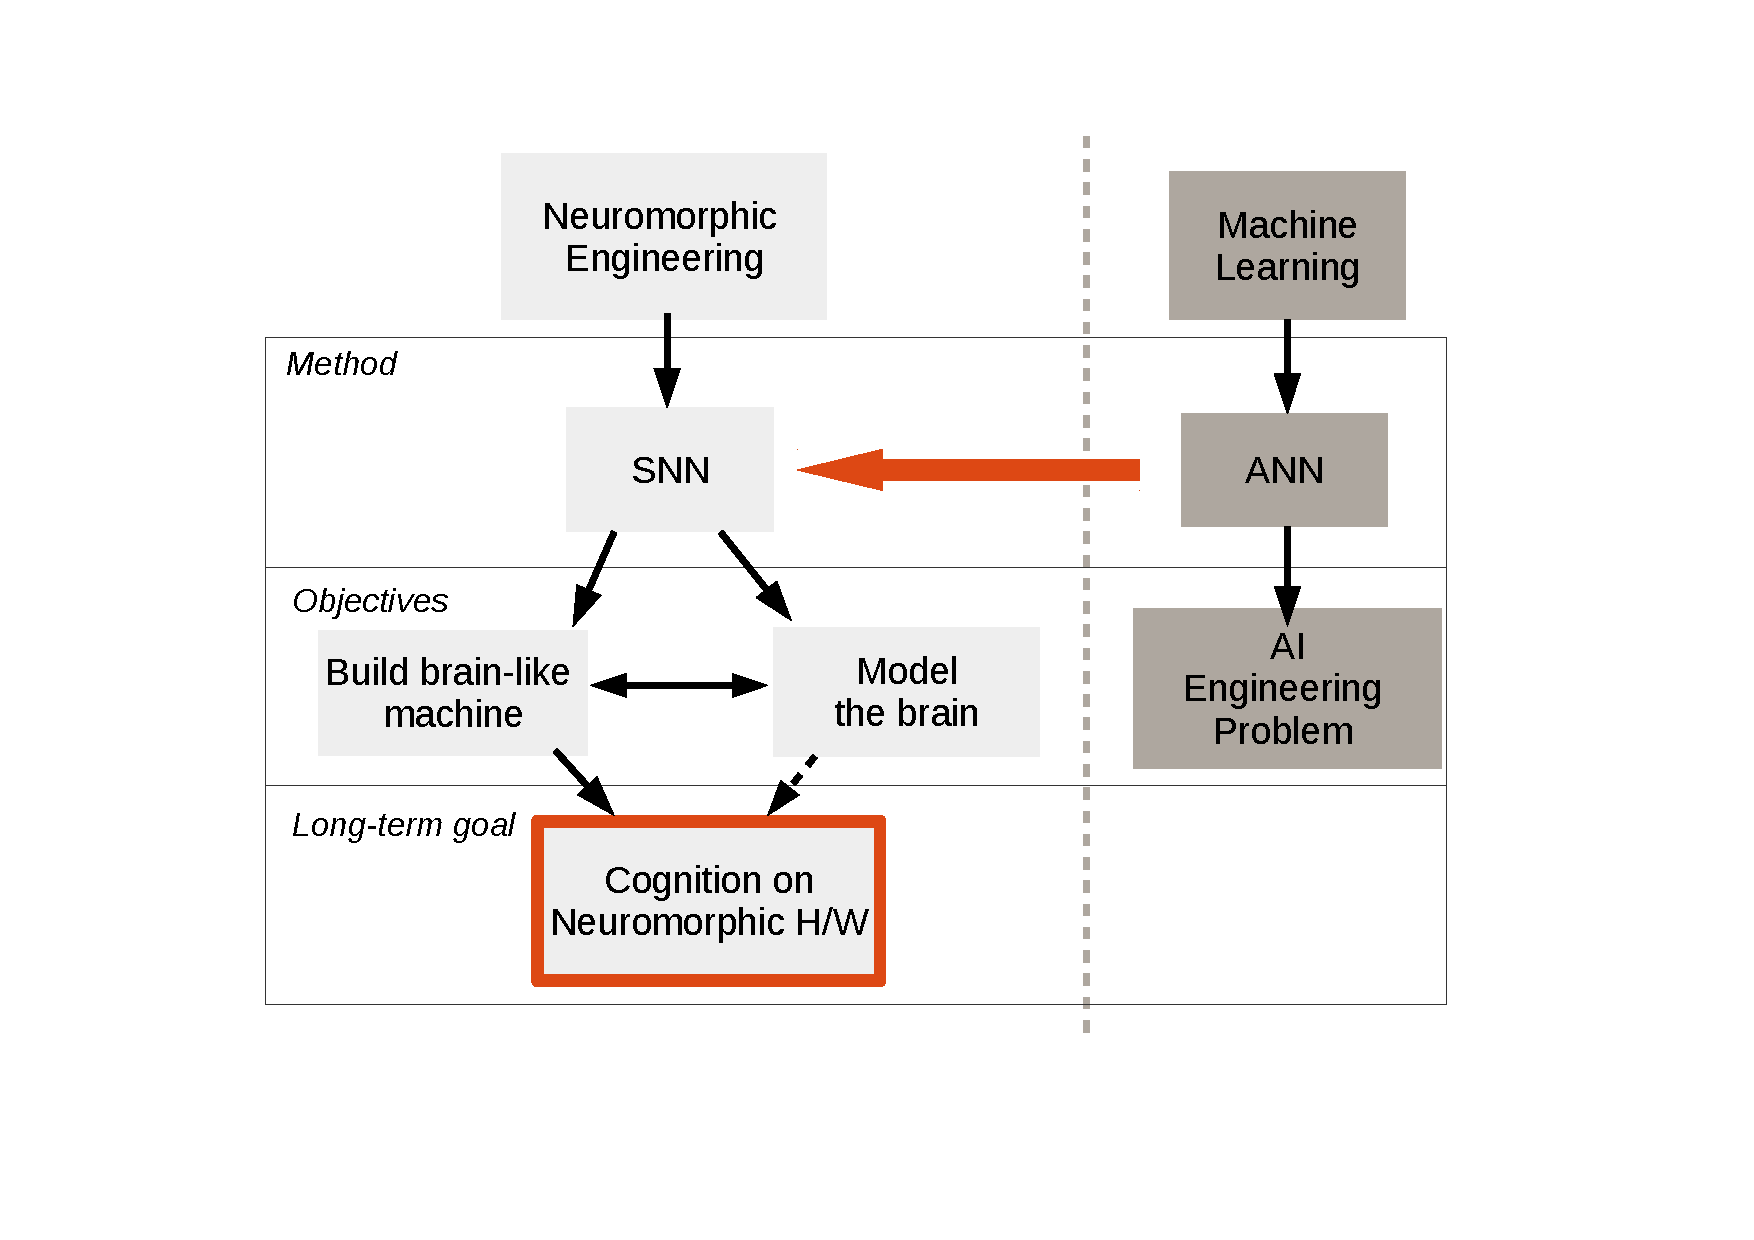
\includegraphics[width=1.0\textwidth]{pics_intro/intro2.pdf}
	\caption{
		The outline of the problem statement of the work.
		%		Neuromorphic engineering and machine learning has been diverging.
		%		This thesis merge the objectives to the ultimate goal of cognition on neuromorphic hardware.
	}
	\label{fig:intro}
\end{figure}




\section{Statement of the Problem}
\label{sec:state_problem}
NE has led to the development of biologically-inspired computer architectures which may provide an alternative to the conventional Von Neumann architecture and achieve the performance of the human brain in terms of energy efficiency and cognitive capabilities.
Although there are a number of neuromorphic platforms available for large-scale SNN simulations, programming these brain-like machines to be competent in cognitive applications still remains unsolved.
On the other hand Deep Learning has emerged in ANN research to dominate state-of-the-art solutions for cognitive tasks.
This raises the main research problem of how to operate and train networks of biologically-plausible spiking neurons to close the gap of cognitive capabilities between SNNs and ANNs in AI tasks.


%Although training SNNs in general is believed to be difficult,  combining deep learning with spiking neurons thus to train SNNs of deep architectures can be simple, effective and generalised because existing approaches have shown promising results in the early stage of the study.

\section{Hypotheses and Aims}
\label{sec:aim}
%The main objective is to improve the cognitive capability of SNNs and equip them with the equivalent learning ability of ANNs for AI applications.
%%In addition, to run such a biologically-plausible model on a complete hardware platform validates the feasibility of real-time Neuromorphic Computing for cognitive tasks.
%Moreover, it is necessary to provide the community with a uniform dataset and an evaluation methodology to compare the performance of SNN models and hardware platforms.
%The goals at this ????? to show that: 


Although fundamental differences in input/output representation and neural computation exist between spiking and conventional artificial neurons, the cognitive capability of SNNs can be improved to catch up with these of ANNs by embedding deep learning techniques in training SNNs, because deep learning has successfully equipped ANNs with better-than-human performance on AI tasks and inspiring work has been reported in training deep SNNs.
Accordingly, the hypotheses and equivalent goals of this thesis are as follows: 
\begin{itemize}
%	\item 
%	An object recognition system can operate in real-time on a complete neuromorphic platform in an absolute spike-based fashion.
%	The hypothesis paves the way for further study with solid proof of the capability of real-time cognitive application built on neuromorphic platform.
%
%	Aim: to build a real-time neuromorphic object recognition prototype running on hardware SNN simulator and receiving visual input from a DVS sensor.

	\item 
%	SNNs can deliver equivalent cognitive capability to conventional ANNs for object recognition applications.
	Deep SNNs can be successfully and simply trained off-line where the training takes place on equivalent ANNs and the trained weights then transferred back to the SNNs, thus making them as competent as ANNs in cognitive tasks. 
	
	Aim: to generalise a training method on conventional ANNs whose trained connections can be transferred to corresponding SNNs to deliver similar recognition performance.

	\item 
	Unsupervised Deep Learning modules can be trained on-line on SNNs with biologically-plausible synaptic plasticity to demonstrate a learning capability as competent as ANNs.

	Aim: to formalise a local learning rule based on synaptic plasticity for unsupervised, event-based, biologically-plausible training of deep SNNs in order to catch up with the recognition performances of ANNs.

	\item 
	A new set of spike-based vision datasets can provide resources to support fair competition between researchers since new concerns relating to energy efficiency and recognition latency emerge in Neuromorphic Vision.

	Aim: to provide a unified spiking version of a commonly-used dataset and a complementary evaluation methodology to assess the performance of SNN algorithms.
\end{itemize}


\section{Contributions}
The primary achievements of the work described in this thesis are the training of deep SNNs, both off-line and on-line, which close the gap of cognitive capability between SNNs and ANNs.
Other achievements contribute to the performance evaluation of SNN models and their hardware implementation.
The contributions are:
\begin{itemize}
%	\item 
%	An implementation of a real-time hand postures recognition system on a neuromorphic hardware platform.
%	It demonstrated the prototype of a complete neuromorphic system which may form the default configuration of a real-time, energy-efficient and low-latency recognition system.
%	
%	This work comprises Chapter 3 and was published and presented to the International Conference on Artificial Neural Networks 2015.
	
	\item 
	a generalised SNN training method to train an equivalent ANN and transfer the trained weights back to SNNs.
	
	This simple method addresses the problems of inaccurate modelling and high computation complexity of existing approaches.
	This training procedure consists of two simple stages: first, estimate parameter $p$ for the Parametric Activation Function~(PAF: $y = p \times f(x)$) using the proposed activation function Noisy Softplus~(NSP), and second, use a PAF version of conventional activation functions for ANN training. % can be generalised to activation units other than NSP.
	%The training of a SNN model is exactly the same as ANN training, and 
	The trained weights can be used directly in the SNN without any further transformation.
	This method requires the least computational complexity while performing most effectively among existing algorithms.

%	A simple and generalised off-line SNN training method which employs a novel activation function, Noisy Softplus.
%	The activation function accurately models the neural response activity of spiking neurons.
%	In addition, it enables an off-line SNN to be trained just like an ANN, and the trained weights can be directly used in SNNs without any conversion.
%	This network training is a generalised method and the activation function can be applied, in principle, in any architecture of a neural network.
%	It was tested on a convolutional network and showed a recognition capability a close to the conventional ANN. 

	NSP is described in Chapter 4 and was published and presented at the International Conference on Neural Information Processing (ICONIP 2016);
	the generalised SNN training using PAF has been submitted to the Annual Conference on Neural Information Processing Systems (NIPS 2017).

	\item 
	an on-line unsupervised learning algorithm working purely on event-based local STDP for training spiking Autoencoders and Restricted Boltzmann Machines.
	
	The proposed Spike-based Rate Multiplication~(SRM) method represents the product of numerical values used in these unsupervised Deep Learning techniques with rate multiplication.
	The SRM then transforms the rate multiplication to the number of coincident spikes emitted from a pair of rate-coded spike trains, and the simultaneous events can be obtained by the biologically-plausible learning rule: Spike-Time-Dependant-Plasticity~(STDP).
	This on-line training method achieves better performance than existing algorithms and approaches the same, sometimes superior performance of the equivalent non-spiking methods.
%	
%	The numerical analysis of the proposed algorithm accurately estimate the configurations of parameters thus to closely mimic the unsupervised learning on these modules and improves the recognition performance of SNNs to reach the ANNs'.
%	The learning ability matched the non-spiking ANNs and verified the feasibility of unsupervised training on deep SNNs. 
	
	This work comprises Chapter 5.
	A paper on these findings is in preparation to submit to Neural Computation.
	
	\item 
	a dataset and the corresponding evaluation methodology for comparisons of Neuromorphic Vision systems.
	
	This dataset aims to (1) promote meaningful comparisons between algorithms in the field of neural computation, (2) allow comparison with conventional image recognition methods, (3) provide an assessment of the state of the art in spike-based visual recognition, and (4) help researchers identify future directions and advance the field.
%	This dataset also made the comparison of SNNs with conventional recognition methods possible by using converted spike representations of the same vision databases.
	As far as we know, this was the first attempt at benchmarking neuromorphic vision recognition by providing a public spike-based dataset and evaluation metrics.
	
	The dataset was generated with the help of Garibaldi Pineda-Garc\'ia and Teresa Serrano-Gotarredona.
%	and the second case study was analysed by Evangelos~Stromatias.
	This work comprises Chapter 6 and was published as a journal paper in Frontiers in Neuromorphic Engineering.
\end{itemize}

   
\section{Papers and Workshops}

\subsection{Papers}
	Much of the work contributed to solving the main research problem of this thesis has either previously been published or been in the process of submission.
\begin{itemize}

	\item 
	\textbf{Q. Liu}, and S. Furber, \textbf{Noisy Softplus: A Biology Inspired Activation Function}, International Conference on Neural Information Processing (ICONIP 2016). 
	This paper~\citep{liu2016noisy} introduces the novel activation function, NSP, 
	which solves the problem of accurately modelling the response firing activity of LIF neurons using conventional abstract activation function.
	This paper comprises the first half of Chapter~\ref{cha:Conv}.
	
	\item 
	\textbf{Q. Liu}, Y. Chen, G. Garc\'ia, and S. Furber, \textbf{Generalised Training of Spiking Neural Networks}, (submitted to NIPS 2017).
	This paper extends the work of the NSP to solve the problem of mapping abstract numerical values of activation functions to concrete physical units in spiking neurons using PAF, and successfully formalises a simple off-line SNN training method which is also generalised to ReLU-like activation functions.
%	This paper extends the work of the NSP to generalise a simple off-line SNN training method using PAF.
	The paper presents the work described in the rest of Chapter~\ref{cha:Conv}.
	
	
	\item 
	\textbf{Q. Liu}, and S. Furber, \textbf{Spike-based Rate Multiplication for On-line SNN Training} (to be submitted to Neural Computation).
	This paper mainly comprises the work of Chapter~\ref{cha:sdlm}, which proposes an on-line unsupervised training of SNNs equivalent to the conventional Deep Learning techniques: AEs and RBMs.
	
	\item 
	\textbf{Q. Liu}, G. Garc\'ia, E. Stromatias, T. Gotarredona, and S. Furber, \textbf{Benchmarking Spike-Based Visual Recognition: A Dataset and Evaluation}, Frontiers in Neuromorphic Engineering.
	The work presented in this paper~\citep{liu2016bench} mainly comprises the spike-based dataset \textbf{NE15-MNIST} and its corresponding evaluation method for Neuromorphic Vision proposed in Chapter~\ref{cha:bench}.
	In addition, the paper also includes the contributions of the co-authors: the detailed description of a subset of this database and a case study as an example to validate the dataset and its evaluation. 
	
\end{itemize}

	Other publications build up the neuromorphic hardware system for complete event-based visual and auditory processing, providing deep spiking neural networks a valid hardware platform for running applications in biologically real time.
\begin{itemize}
	\item 
	\textbf{Q. Liu}, and S. Furber, \textbf{Real-Time Recognition of Dynamic Hand Postures on a Neuromorphic System}, International Conference on Artificial Neural Networks (ICANN 2015).
	We develop an object recognition system operating in real-time on a complete neuromorphic platform in an absolute spike-based fashion.
	This paper paves the way for further study with solid proof of the capability of real-time cognitive application built on neuromorphic platform.
	In Chapter~~\ref{cha:bkg}, we introduce this system as an existing vision-based neuromorphic hardware platform which comprises a Dynamic Vision Sensor~(DVS) as front-end and a massive-parallel SNN hardware simulator as the back-end. 
	
	\item
	\textbf{Q. Liu}, C. Patterson, S. Furber, Z. Huang, Y. Hou and H. Zhang, \textbf{Modeling Populations of Spiking Neurons for Fine Timing Sound Localization}, International Joint Conference on Neural Networks (IJCNN 2013)
	This paper~\citep{liu2013modeling} presents a model of sound localisation to solve the problem of coarse time resolution of SNN simulations.
	Such an auditory processing system can be implemented on a similar neuromorphic hardware platform described above, which uses a silicon cochlea as the input (see Chapter~\ref{cha:bkg}).
	
	\item 
	G. Garc\'ia, P. Camilleri, \textbf{Q. Liu}, and S. Furber, \textbf{pyDVS: An Extensible, Real-time Dynamic Vision Sensor Emulator using Off-the-Shelf Hardware}, The 2016 IEEE Symposium Series on Computational Intelligence (IEEE SSCI 2016).
	This paper~\citep{7850249} proposes a visual input system inspired by the behaviour of a DVS but using a conventional digital camera as a sensor and a
	PC to encode the images.
	We mentioned the neuromorphic input sensors in Chapter~\ref{cha:bkg}).
\end{itemize}


\subsection{Workshops}
The author participated in workshops organised by the community, 1) to establish and contribute to collaborations on mutual interests; 2) to catch up with cutting-edge research and collect inspiration; 3) to discuss the author's own findings with key researchers in the field.
\begin{itemize}
	\item 
	\textit{Capo Caccia Cognitive Neuromorphic Engineering Workshop 2012}.
	
	Contributed to successful connections of SpiNNaker to neuromorphic sensors\footnote{\url{https://capocaccia.ethz.ch/capo/wiki/2012/csnQian}}. 
	This formed the hardware platform for real-time SNN applications processing event-based sensor data.
	
	\item 
	\textit{Telluride Neuromorphic Cognition Engineering Workshop 2013}.
	
	Developed a real-time sound localisation system on the neuromorphic platform as a main contributor\footnote{\url{http://neuromorphs.net/nm/wiki/sound_localization}}.
	The work led to the publication of a journal paper~\citep{lagorce2015breaking}.
	
	
	\item 
	\textit{Capo Caccia Cognitive Neuromorphic Engineering Workshop 2014}.
	
	Developed the real-time neural activity visualiser for the project of `Integrated Neurorobotics for Real-World Cognitive Behaviour' \footnote{\url{https://capocaccia.ethz.ch/capo//wiki/2014/integrneurobot14}}. 
	
	\item 
	\textit{Capo Caccia Cognitive Neuromorphic Engineering Workshop 2015}.
	
	Inspired by the projects on deep learning in the workshop\footnote{\url{https://capocaccia.ethz.ch/capo//wiki/2015/spikednn15}}, the author later proposed the translation methods and the unsupervised learning algorithm of spiking deep networks, and led the discussion of benchmarking neuromorphic vision in the workshop \footnote{\url{https://capocaccia.ethz.ch/capo//wiki/2015/visionbenchmark15}}. 	
\end{itemize}
\section{Thesis Structure}
The thesis comprises the following seven chapters:

\textbf{Chapter 1} introduces the origin and the motivation of the research, states the problem, defines the hypotheses and objectives, summarises the contributions and publications, and outlines the thesis. 

\textbf{Chapter 2} %briefs the short history	 of Neuromorphic Engineering which leads to the author's research, lists the common spiking neural models and learning approaches, introduces the neuromorphic hardware devices.
illustrates how biological neurons function, transmit signals between them, and are modelled by mathematical abstractions, thus to unveil the special features of spiking neurons that differ from the neurons of ANNs; and introduces SNN simulators both in software and in hardware including neuromorphic systems.

\textbf{Chapter 3} gives an overview of popular architectures and models of Deep Learning and illustrates the mechanism of the convolutional network~(ConvNet), the Autoencode~(AE), and the Restricted Boltzmann Machine~(RBM) in detail.

\textbf{Chapter 4} demonstrates the generalised off-line SNN training method by using a novel biologically-inspired activation function, Noisy Softplus, which is well-matched to the response function of Leaky Integrate-and-Fire neurons; and validates the performance by testing on a convolutional network.

\textbf{Chapter 5} proposes the STDP-based learning algorithm for training spiking AEs and RBMs; and shows equivalent recognition capability of SNNs compared to ANNs.

\textbf{Chapter 6} puts forward the spike-based vision dataset and the evaluation methodology; and presents two case studies as tentative benchmarks running on SpiNNaker to assess the hardware-level performance against software simulators.

\textbf{Chapter 7} summarises the research, discusses the contributions to the field, points out future directions and concludes the thesis.



